\section{Functionality}
\label{sec:features}

For each feature:
\begin{itemize}
\item{Description}
\item{Implementation}
\item{Why is it useful?}
\item{Minimal example}
\end{itemize}

\subsection{Integrated Scripting}

In order for a theorem prover to be truly useful, it is not sufficient to be
able to answer 'true' or 'false' given an input formula. Rather, our
experience has shown that students will need to formulate and extend theories.
Doing this by hand by editing a single large formula quickly becomes
unmanageable.
Moreover, we want to have a powerful toolbox to assist us in the formulation
of larger theories, often including general programming constructs such as
loops and conditionals. Some other tools, such as the LWB, provide custom
scripting languages for this purpose. The advantage of this approach is that
the language can be tailored specifically to common usage of the prover. The
disadvantage, however, is that developing a custom language is costly.
Therefore, that the resulting language is likely to be lacking in expressive
power. Furthermore, the user has to learn a language that has no application
outside of the prover and for which support may be limited.

To address these concerns, \oops\ integrates the
luaj\footnote{http://luaj.sourceforge.net/} pure Java implementation of the
Lua\footnote{http://www.lua.org/} general-purpose scripting language. Lua has
been designed specifically to be an embeddable language and is widely used
both as an extension language and as a front-end for libraries written in
other languages. Currently, most of \oops' functionality is available from
Lua and more extensive support is being worked on.

FIXME: explain specifics, give example

\subsection{Graphical User Interface}

\oops\ includes a very simple Graphical User Interface (GUI), in which scripts
can be displayed, edited and executed (Figure~\ref{fig:gui}). In addition,
scripts can be loaded from and saved to a file. For those who prefer to use an
external editor (e.g., there are many editors that offer syntax highlighting
for Lua), a single key combination reloads a modified file from the
file system. The application consists of two panels: the top panel shows the
script that is currently being worked on and the bottom panel shows the
output.

\begin{figure}
\centering
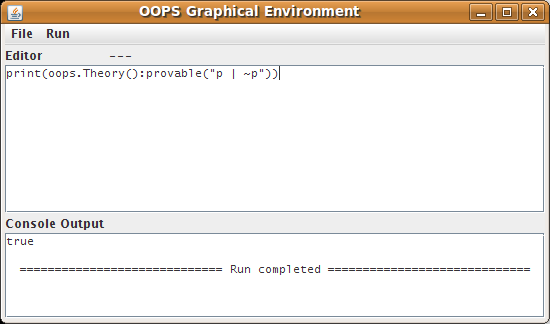
\includegraphics[width=0.7\textwidth]{images/gui}
\caption{The \oops\ Graphical User Interface}
\label{fig:gui}
\end{figure}

Though minimal, the GUI greatly enhances the convenience with which \oops\ can
be used. Firstly, script and output are shown in one place, allowing for easy
cross-referencing. Second, scripts are run through a single key combination
(or invocation from the menu). Finally, load, save and refresh functionality
gives the user the freedom to use the integrated editor or an external editor
of choice with equal convenience.

\subsection{Free and Convenient Distribution}

As we noted in Section~\ref{sec:introduction}, most current proof tools have
problems related to either platform dependence, aging dependencies, lack of
maintenance or difficult installation procedures. \oops\ addresses these
problems in several ways. First, \oops\ is implemented in pure Java, which
means that \oops\ will run on any operating system for which a Java virtual
machine is available. This is true for most operating systems. Second, \oops\
is distributed as a ZIP file that includes all dependencies. No installation
is needed, one simply extracts the ZIP file and double-clicks the resulting
{\texttt oops.jar} file. Hence, \oops\ is platform independent and easy to
run, having no dependencies apart from the Java VM and what is provided in the
\oops\ distribution.

The concern of continued maintenance is harder to address. To ensure that
\oops\ can be used and extended in the future, by anyone who wishes to do so,
we provide the full source code\footnote{http://github.com/gertvv/oops} under
the GNU General Public License (GPL). It is our hope that others will
contribute extensions to \oops.

\subsection{Visualization of Tableaux}

When learning to work with modal logics, a prover can often give surprising
results. The student may encounter undesirable outcomes when constructing a
theory and would like to be able to `debug' the theory by inspecting the proof
process. Moreover, inspecting generated tableaux may enhance understanding of
tableau methods and the semantics of modal logics in general.
To support this, oops includes a visualization module for labeled tableaux.
Figure~FIXME shows an example of such a visualization. 

FIXME: figure

The visualization is implemented as an observer on the tableau generator,
using the provided hooks (Section~FIXME). FIXME: etc

\subsection{Visualization of Counter Models}

\subsection{Interchangeable Rule Sets}

